\newcommand{\neuron}[3]{\draw[fill, white] (#1, #2) circle (0.5); \draw (#1, #2) circle (0.5) node {#3};}

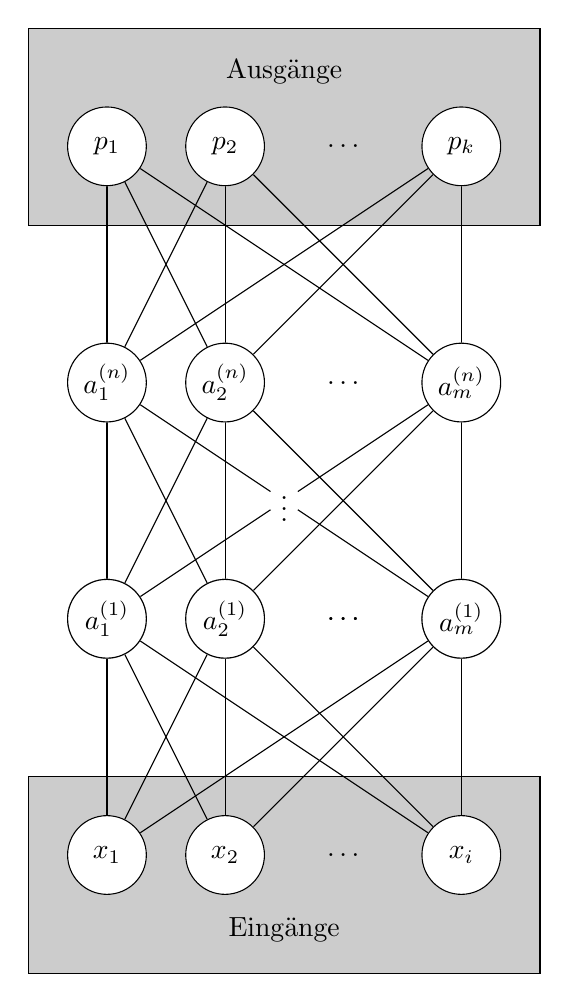
\begin{tikzpicture}
	\draw[fill=black!20] (-1, -1.5) rectangle (5.5, 1) node[midway, yshift=-20] {Eingänge};
	\draw[fill=black!20] (-1, 10.5) rectangle (5.5, 8) node[midway, yshift=20] {Ausgänge};

	% Verbindungen
	\draw (0, 3) -- (0, 0);
	\draw (0, 3) -- (1.5, 0);
	\draw (0, 3) -- (4.5, 0);
	\draw (1.5, 3) -- (0, 0);
	\draw (1.5, 3) -- (1.5, 0);
	\draw (1.5, 3) -- (4.5, 0);
	\draw (4.5, 3) -- (0, 0);
	\draw (4.5, 3) -- (1.5, 0);
	\draw (4.5, 3) -- (4.5, 0);
	
	\draw (0, 6) -- (0, 3);
	\draw (0, 6) -- (1.5, 3);
	\draw (0, 6) -- (4.5, 3);
	\draw (1.5, 6) -- (0, 3);
	\draw (1.5, 6) -- (1.5, 3);
	\draw (1.5, 6) -- (4.5, 3);
	\draw (4.5, 6) -- (0, 3);
	\draw (4.5, 6) -- (1.5, 3);
	\draw (4.5, 6) -- (4.5, 3);
	
	\draw (0, 9) -- (0, 6);
	\draw (0, 9) -- (1.5, 6);
	\draw (0, 9) -- (4.5, 6);
	\draw (1.5, 9) -- (0, 6);
	\draw (1.5, 9) -- (1.5, 6);
	\draw (1.5, 9) -- (4.5, 6);
	\draw (4.5, 9) -- (0, 6);
	\draw (4.5, 9) -- (1.5, 6);
	\draw (4.5, 9) -- (4.5, 6);
	
	% Eingänge
	\neuron{0}{0}{$x_1$}
	\neuron{1.5}{0}{$x_2$}
	\draw (3, 0) node {$\dots$};
	\neuron{4.5}{0}{$x_i$}
	
	% 1. Layer
	\neuron{0}{3}{$a_1^{(1)}$}
	\neuron{1.5}{3}{$a_2^{(1)}$}
	\draw (3, 3) node {$\dots$};
	\neuron{4.5}{3}{$a_m^{(1)}$}
	
	\draw[fill, white] (4.5 / 2, 4.5) circle (0.2);
	\draw (4.5 / 2, 4.5) node {$\vdots$};
	
	% 1. Layer
	\neuron{0}{3}{$a_1^{(1)}$}
	\neuron{1.5}{3}{$a_2^{(1)}$}
	\draw (3, 3) node {$\dots$};
	\neuron{4.5}{3}{$a_m^{(1)}$}
	
	% n. Layer
	\neuron{0}{6}{$a_1^{(n)}$}
	\neuron{1.5}{6}{$a_2^{(n)}$}
	\draw (3, 6) node {$\dots$};
	\neuron{4.5}{6}{$a_m^{(n)}$}
	
	% Ausgänge
	\neuron{0}{9}{$p_1$}
	\neuron{1.5}{9}{$p_2$}
	\draw (3, 9) node {$\dots$};
	\neuron{4.5}{9}{$p_k$}
\end{tikzpicture}